\subsection{アクリル樹脂(PMMA)}
アクリル樹脂(PMMA)はハイブリッドロケットの燃料として多くの実績があり、また非常に高い透明性があるため、
本実験で用いる燃料はアクリル樹脂(PMMA)とした。PMMAの写真を図\ref{fig:PMMA}に示す。
PMMAは円筒形になっており長さの違う3つの形状を製作した。表\ref{tab:PMMA}に示す。

\begin{figure}[htbp]
\centering
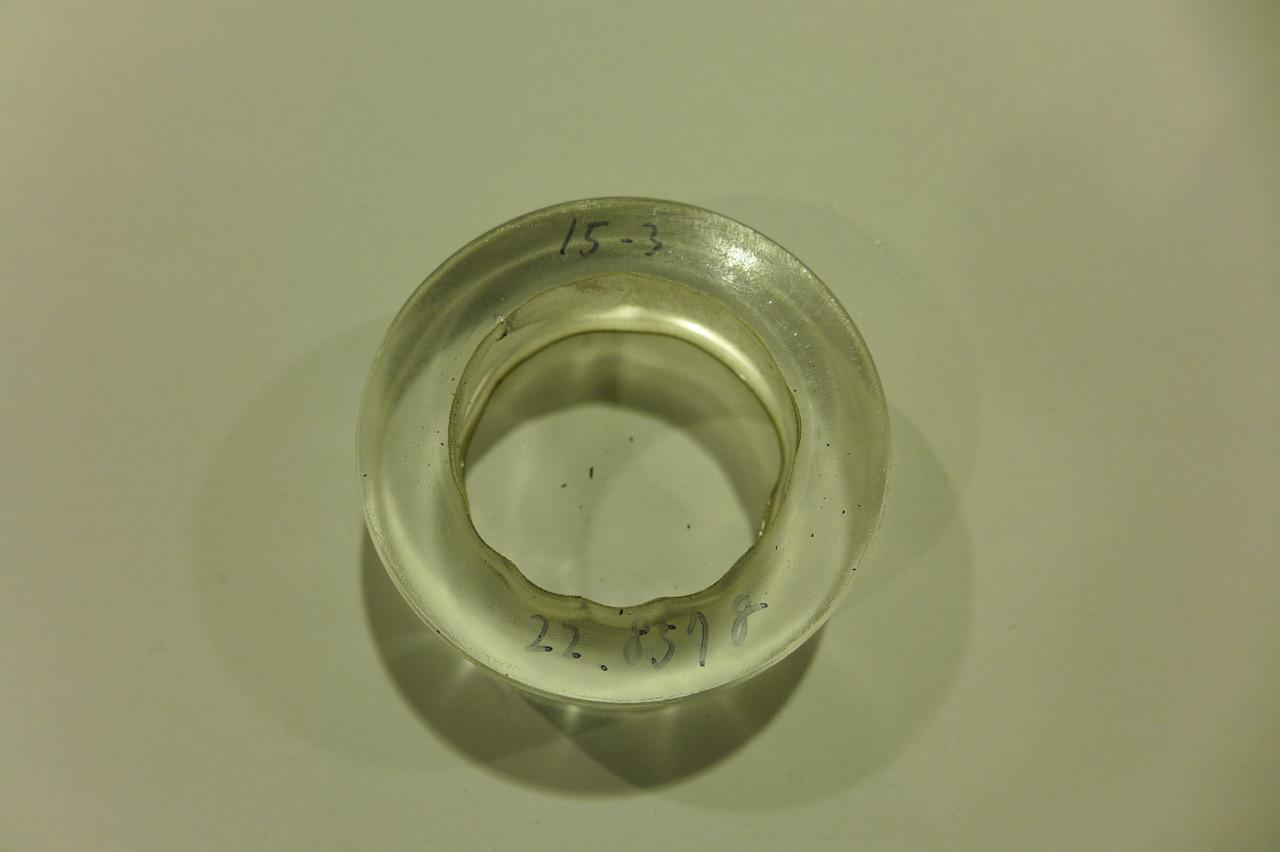
\includegraphics[width=10cm]{\FigAddTwo/PMMA.jpg}
\caption{PMMA}
\label{fig:PMMA}
\end{figure}

\begin{table}[htb]
\begin{center}
\caption{PMMA形状}
\begin{tabular}{|l|c|c|c|} \hline
 & 長さ  & 外径 & 内径\\ \hline
1 & 30  &  & \\ \cline{1-2}
2 & 15  & 50 & 30\\ \cline{1-2}
3 & 7.5 &  &  \\ \hline
\end{tabular}
\label{tab:PMMA}
\end{center}
\end{table}

